\documentclass[a0paper, fleqn]{tikzposter}

\title{Machine-Checked C Implementation of Dijkstra}
\author{\underline{Anshuman Mohan} \hspace{2ex} Aquinas Hobor}
\institute{National University of Singapore}
\usetheme{Simple}
\usepackage{fontspec}
\defaultfontfeatures{Mapping=tex-text,Scale=MatchLowercase}
% \setmainfont{Minion Pro}
% \setsansfont{Myriad Pro}
% \setmonofont{Source Code Pro}

\colorlet{red}{green!30!black}
\colorlet{titlebgcolor}{red}
\colorlet{blocktitlefgcolor}{red}
\colorlet{maincolor}{titlebgcolor}
\colorlet{accentcolor}{titlebgcolor!40!white}
\usepackage{amsmath, amssymb, mathabx}
\usepackage{mathpartir}        % for inferrule
\usepackage{listings}
\usepackage{mathtools}         % for mathrlap
\usepackage{caption}
\usepackage{multicol}          % for multi-column listings  
\usepackage{stmaryrd}          % for the lightning symbol
\usepackage{fancyvrb}
\usepackage{scalerel}


\makeatletter
\newlength{\@mli}
\newcommand\hide[1]{}
\newcommand{\mli}[1]{%
  \settowidth{\@mli}{\lstinline/#1/}
  \hspace{-.5ex}\begin{minipage}[t]{\@mli}\lstinline/#1/\end{minipage}}
\makeatother
\newcommand{\li}[1]{\ifmmode\mbox{\mli{#1}}\else\mbox{\lstinline/#1/}\fi}
\newcommand{\infrulestyle}[1]{\textsc{#1}}
% \newcommand{\infrule}[4]{\inferrule*[lab=\infrulestyle{#1},right=$\mathrlap{#4}$]{#2}{#3}}

\newcommand{\hl}[1]{\colorbox{lightgray}{#1}}
\newcommand{\tx}[1]{\text{#1}}
\newcommand{\p}[1]{\ensuremath{\mathsf{#1}}} % predicate font
\newcommand{\m}[1]{\ensuremath{\mathit{#1}}} % math font
\newcommand{\braces}[1]{\left\{\begin{array}{l@{}} #1 \end{array}\right\}}
\let\ramify\lightning
\newcommand{\sz}{\texttt{SIZE}}
\newcommand{\ifty}{\texttt{INF}}

\lstset{%
  language=C,
  sensitive=true,
  mathescape=true,
  showlines=true,
  basicstyle=\normalfont\tt,
  keywordstyle=\color{blocktitlebgcolor},
  numbers=left,
  numberstyle=\small,
  numbersep=5pt,
  boxpos=t,
}

\usepackage[style=numeric]{biblatex}
\addbibresource{poster.bib}

\usepackage{semantic}
\newcommand{\scon}{\mathbin{\ast}}
\renewcommand{\bigstar}{\raisebox{-0.24em}{{\scaleobj{2.5}{\scon}}}}

\newcommand{\ocon}{%
  \mathbin{\mbox{$\mathrlap{\cup}\hspace*{.15em}
      \raisebox{.01em}[0ex][0ex]{$\scon$}$\hspace*{.07em}}}}
\newcommand{\wand}{%
 \mathrel{\mbox{$\hspace*{-0.03em}\mathord{-}\hspace*{-0.4em}
  \mathord{-}\hspace*{-0.13em}
     \mathord{\scon}$\hspace*{-0.005em}}}}
\newcommand{\septraction}{%
  \mathrel{\mbox{$\hspace*{-0.03em}\mathord{-}\hspace*{-0.66em}
  \mathord{-}\hspace*{-0.155em}\mathord{\ocircle\hspace*{-.66em}\scon}$\hspace*{0.05em}}}}
\newcommand{\magicwand}{\wand}
\newcommand{\defeq}{\mathbin{\stackrel{\Delta}{=}}}
\newcommand{\MV}{\ensuremath{\mathsf{ModVar}}}
\newcommand{\FV}{\ensuremath{\mathsf{FreeVar}}}
\newcommand{\bigocon}{
  \raisebox{-0.3ex}{\resizebox{0.75em}{!}{$\scon$}} \hspace{-4.3ex} \bigcup}
\newcommand{\medocon}{
  \raisebox{-0.3ex}{\resizebox{0.63em}{!}{$\scon$}} \hspace{-2.05ex} \bigcup}
  \newcommand{\reachable}[5]{\ensuremath{{\m{#1}\; \stackrel{#2}{\leadsto}^{#3}_{#4} \m{#5}}}}


%\input mathlig
\mathlig{--*}{\mathrel{\magicwand}}
\mathlig{--o}{\mathrel{\septraction}}
\mathlig{|->}{\mathrel{\mapsto}} % tight points-to
\mathlig{<=>}{\mathrel{\Leftrightarrow}} % equivalence of expressions
\mathlig{==>}{\mathrel{\Rightarrow}} % meta implication
\mathlig{-|-}{\mathrel{\mathrlap{\dashv} \hspace{5pt} \vdash}} % entails

\mathlig{/|}{\mathbin{\wedge}} % additive conjunction
\mathlig{|/}{\mathbin{\vee}} % additive disjunction
\mathlig{|-}{\mathrel{\vdashtwo}} % entails
\mathlig{|=}{\vDash} % models

\mathlig{**}{\mathbin{\ocon}}
\mathlig{*}{\mathbin{\scon}}
\mathlig{//}{\color{maincolor}{//}} % listings comments


\usepackage{tikz}
\usepackage{xcolor}
\usetikzlibrary{shadows}
\usetikzlibrary{arrows.meta, positioning, decorations.pathmorphing, fit, matrix}
\colorlet{backgroundcolor}{white}
% \titlebgcolor{\color{red}}
% \subsectionfont{\color{red}}
% \sectionfont{\color{red}}

\begin{document}
\maketitle

% \begin{tikzpicture}
     % \node [anchor=north east, inner sep=3cm]  at (current page.north east)
     % {\includegraphics[scale=0.3]{badges}};
  % \end{tikzpicture}
\begin{columns}
  \column{0.5}
  \block{Overview}{%
We report on a machine-checked proof of correctness
for Dijkstra's one-to-all shortest path algorithm.
Unlike previous work, we use classic textbook code
written in executable C~\cite{clrs}.

\vspace{0.5em}

\textbf{Challenges:} 
We use CompCert C, which is executable and realistic but also has real-world complications.
We prove full functional correctness, and not just program safety.

\vspace{0.5em}

\textbf{Solution:} We use the Verified Software Toolchain~\cite{appel:vst} and 
our Mathematical and Spatial Graph Libraries~\cite{wang:autoquack} to establish machine-checked
correctness at the C level ($3$ files, $3$k \textsc{loc}). 
The CompCert compiler~\cite{leroy:compcert} then guarantees this correctness on the executable code.

\vspace{0.5em}

\textbf{Key findings:} 
The algorithm suffers from potential overflow issues. 
The precise bound is nontrivial: we show that the intuitive 
guess fails, and provide a workable refinement.
\vspace{-1.5em}
}%end block


\block{Workflow}{A sketch of how we verify C programs. Note where we 
integrate with other projects.

\vspace{0.5em}

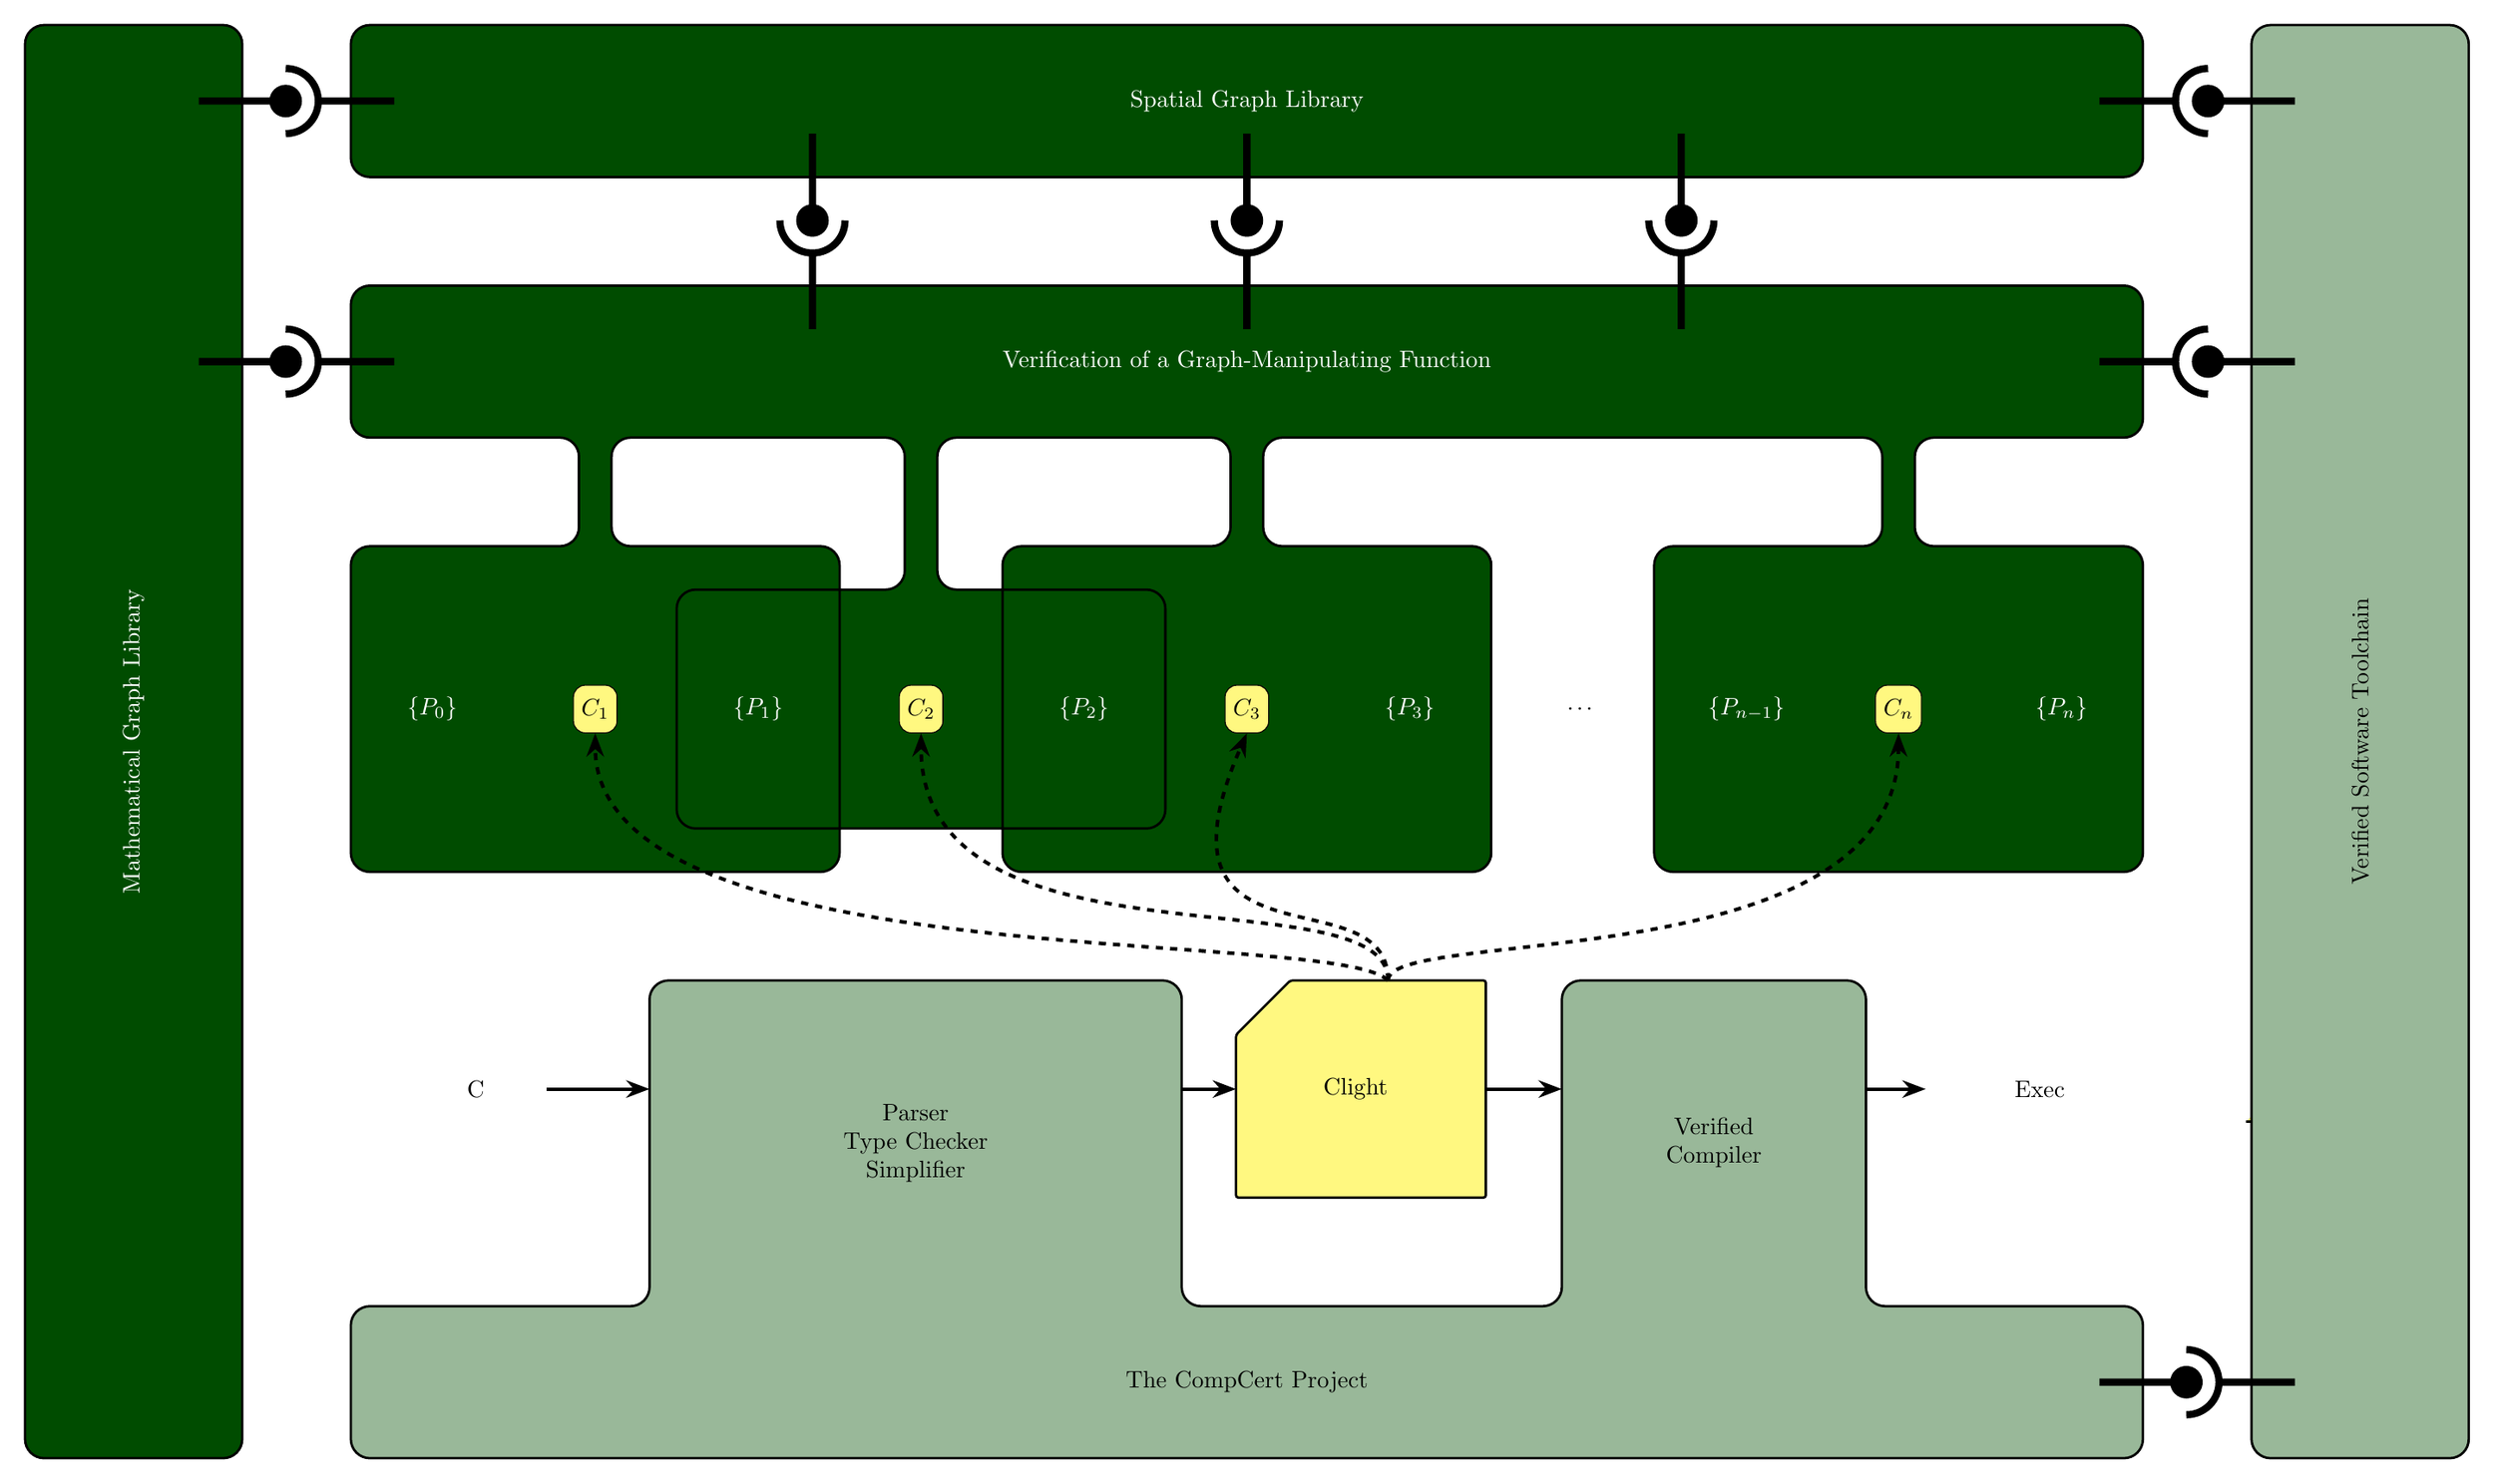
\begin{tikzpicture}[on grid, cmd/.style={rectangle, fill=yellow!50!white, minimum width=2em, minimum height=1em, draw=black, rounded corners=5pt},
  ourlib/.style={rounded corners=8pt, line width=1pt},
  test/.style={rounded corners=8pt, draw=red},
  file/.style={rounded corners=1pt, line width=1pt, fill=yellow!50!white},
  ->/.style={-Stealth, line width=1.5pt}, rotate=90,transform shape, x=1.6cm, y=1.6cm]
  %% \draw [test] (-1.5, -0.5) rectangle (1.5, 2.5);
  %% \draw [test] (-1.5, 3.5) rectangle (1.5, 6.5);
  %% \draw [test] (-1.1, 5.5) rectangle (1.1, 8.5);
  %% \draw [test] (-1.5, 7.5) rectangle (1.5, 10.5);
  \draw [ourlib, fill=maincolor] (-1.5, -0.75) -- ++(3, 0) -- ++(0, 2.1) -- ++(1, 0) -- ++(0, -2.1) -- ++(1.4, 0) -- ++(0, 16.5) -- ++(-1.4, 0) --
  ++(0, -2.1) -- ++(-1, 0) -- ++(0, 2.1) -- ++(-3, 0) -- ++(0, -4.5) -- ++(3, 0) -- ++(0, 2.1) -- ++(1, 0) -- ++(0, -2.7) -- ++(-1.4, 0) -- ++(0, 2.1) --
  ++(-2.2, 0) -- ++(0, -4.5) -- ++(2.2, 0) -- ++(0, 2.1) -- ++(1.4, 0) -- ++(0, -2.7) -- ++(-1, 0) -- ++(0, 2.1) -- ++(-3, 0) -- ++(0, -4.5) -- ++(3, 0)
  -- ++(0, 2.1) -- ++(1, 0) -- ++(0, -5.7) -- ++(-1, 0) -- ++(0, 2.1) -- ++(-3, 0) -- cycle;
  \node (Pn) at (0, 0) {\rotatebox{-90}{\color{white}$\{P_n\}$}};
  \node (Pn1) [above=2.9 of Pn]  {\rotatebox{-90}{\color{white}$\{P_{n-1}\}$}};
  \node (etc) [above=1.6 of Pn1] {\vdots};
  \node (P3) [above=1.5 of etc]  {\rotatebox{-90}{\color{white}$\{P_3\}$}};
  \node (P2) [above=3 of P3]  {\rotatebox{-90}{\color{white}$\{P_2\}$}};
  \node (P1) [above=3 of P2]  {\rotatebox{-90}{\color{white}$\{P_1\}$}};
  \node (P0) [above=3 of P1]  {\rotatebox{-90}{\color{white}$\{P_0\}$}};
  \node (Cn) [above=1.5 of Pn] [cmd] {\rotatebox{-90}{$C_n$}};
  \node (C3) [above=1.5 of P3] [cmd] {\rotatebox{-90}{$C_3$}};
  \node (C2) [above=3 of C3] [cmd] {\rotatebox{-90}{$C_2$}};
  \node (C1) [above=3 of C2] [cmd] {\rotatebox{-90}{$C_1$}};

  % If I uncomment this line I get the "file", but I also get a yellow triangle below the figure.
  % I have tried various tricks to get it to go away but I can't seem to figure it out.
  % \draw [file] (-4.5, 13.95) -- ++(2, 0) -- ++ (0, 1.5) -- +(-0.5, 0.5) -- +(-2, 0.5) -- cycle ++(2, 2.3) -- ++(-0.5, 0) -- ++(0, 0.5);

  \draw [file] (-4.5, 05.30) -- ++(2, 0) -- ++ (0, 1.8) -- +(-0.5, 0.5) -- +(-2, 0.5) -- cycle ++(2, 2.3) -- ++(-0.5, 0) -- ++(0, 0.5);
  
  % \draw [file] (-4.5, -0.75) -- ++(2, 0) -- ++ (0, 1.5) -- +(-0.5, 0.5) -- +(-2, 0.5) -- cycle ++(2, 2.3) -- ++(-0.5, 0) -- ++(0, 0.5);
  
  \node at (-3.5, 14.6) {\rotatebox{-90}{C}};
  \node at (-3.5, 6.5) {\rotatebox{-90}{Clight}};
  \node at (-3.5, 0.2) {\rotatebox{-90}{Exec}};
  \draw [->, dashed] (-2.5, 6.2) .. controls ++(0.5, 0.5) and (-2.5, 13.5) .. (C1.west);
  \draw [->, dashed] (-2.5, 6.2) .. controls ++(1, 0) and (-2.5, 10.5) .. (C2.west);
  \draw [->, dashed] (-2.5, 6.2) .. controls ++(1, 0) and (-2.5, 8.5) .. (C3.west);
  \draw [->, dashed] (-2.5, 6.2) .. controls ++(0.5, 0) and (-2.5, 1.5) .. (Cn.west);
  \draw [->] (-3.5, 13.95) -- (-3.5, 13.0);
  \draw [->] (-3.5, 12) -- (-3.5, 7.6);
  \draw [->] (-3.5, 5.3) -- (-3.5, 4.6);
  \draw [->] (-3.5, 4.5) -- (-3.5, 1.25);
  %% \draw [test] (-6.9, -0.75) rectangle (-5.5, 15.75);
  %% \draw [test] (-4.2, 9.9) rectangle (-2.8, 11.95);
  %% \draw [test] (-4.2, 3.05) rectangle (-2.8, 5.1);
  \draw [ourlib, fill=accentcolor] (-6.9, -0.75) -- (-5.5, -0.75) -- (-5.5, 1.8) -- (-2.5, 1.8) -- (-2.5, 4.6) -- (-5.5, 4.6) -- (-5.5, 8.1) --
  (-2.5, 8.1) -- (-2.5, 13.0) -- (-5.5, 13) -- (-5.5, 15.75) -- (-6.9, 15.75) -- cycle;
  \node at (-4, 10.55) {\rotatebox{-90}{\begin{tabular}{c} Parser\\ Type Checker \\ Simplifier \end{tabular}}};
  \node at (-4, 3.2) {\rotatebox{-90}{\begin{tabular}{c} Verified \\ Compiler \end{tabular}}};
  \node at (-6.2, 7.5) {\rotatebox{-90}{The CompCert Project}};
  \draw [ourlib, fill=accentcolor] (-6.9, -3.75) rectangle (6.3, -1.75);
  \node at (-0.3, -2.75) {Verified Software Toolchain};
  \draw [ourlib, fill=maincolor] (-6.9, 16.75) rectangle (6.3, 18.75);
  \node at (-0.3, 17.75) {\color{white}Mathematical Graph Library};
  \node at (3.2, 7.5) {\rotatebox{-90}{\color{white}Verification of a Graph-Manipulating Function}};
  \draw [ourlib, fill=maincolor] (4.9, -0.75) rectangle (6.3, 15.75);
  \node at (5.6, 7.5) {\rotatebox{-90}{\color{white}Spatial Graph Library}};

  %% down interface
  \draw [line width=3pt] (5.6, -0.35) -- +(0, -0.7) +(0, -1.05) -- +(0, -1.8) +(0.3, -1) arc [start angle=0, end angle=180, radius=0.3];
  \fill (5.6, -1.35) circle [radius=0.15];
  \draw [line width=3pt] (3.2, -0.35) -- +(0, -0.7) +(0, -1.05) -- +(0, -1.8) +(0.3, -1) arc [start angle=0, end angle=180, radius=0.3];
  \fill (3.2, -1.35) circle [radius=0.15];

  %% up interface
  \draw [line width=3pt] (-6.2, -2.15) -- +(0, 0.7) +(0, 1.05) -- +(0, 1.8) +(0.3, 1) arc [start angle=0, end angle=-180, radius=0.3];
  \fill (-6.2, -1.15) circle [radius=0.15];
  \draw [line width=3pt] (3.2, 15.35) -- +(0, 0.7) +(0, 1.05) -- +(0, 1.8) +(0.3, 1) arc [start angle=0, end angle=-180, radius=0.3];
  \fill (3.2, 16.35) circle [radius=0.15];
  \draw [line width=3pt] (5.6, 15.35) -- +(0, 0.7) +(0, 1.05) -- +(0, 1.8) +(0.3, 1) arc [start angle=0, end angle=-180, radius=0.3];
  \fill (5.6, 16.35) circle [radius=0.15];

  %% right interface
  \draw [line width=3pt] (3.5, 7.5) -- +(0.7, 0) +(1.05, 0) -- +(1.8, 0) +(1, 0.3) arc [start angle=90, end angle=270, radius=0.3];
  \fill (4.5, 7.5) circle [radius=0.15];
  \draw [line width=3pt] (3.5, 11.5) -- +(0.7, 0) +(1.05, 0) -- +(1.8, 0) +(1, 0.3) arc [start angle=90, end angle=270, radius=0.3];
  \fill (4.5, 11.5) circle [radius=0.15];  
  \draw [line width=3pt] (3.5, 3.5) -- +(0.7, 0) +(1.05, 0) -- +(1.8, 0) +(1, 0.3) arc [start angle=90, end angle=270, radius=0.3];
  \fill (4.5, 3.5) circle [radius=0.15];
\end{tikzpicture}

\vspace{-1.5em}}

  % \block{}{\centering\begin{tabular}{c|c|c|c|c}
Component & Files & Size (loc) & Definitions & Theorems\\\hline
Common Utilities & 10 & 3,578 & 44 & 289 \\
Math Graph Library &  20 & 10,585 & 216 & 581 \\
Spatial Graph Library &  3 & 2,328 & 59 & 110 \\
Integration into VST & 11 & 2,783 & 17 & 172 \\
\hline
Marking (graph and DAG) &  6 & 775 & 9 & 20 \\
Spanning Tree & 5 & 2,723 & 17 & 92 \\
Union-Find (heap and array) &  18 & 3,193 & 107 & 135 \\
Garbage Collector & 16 & 13,858 & 235 & 712 \\
% \hline & & & &  \\
% [-2.2em] \\
% \hline & & & & \\
\hline
Total Development & 89 & 39,823 & 704 & 2,111 \\
\end{tabular}
\hide{
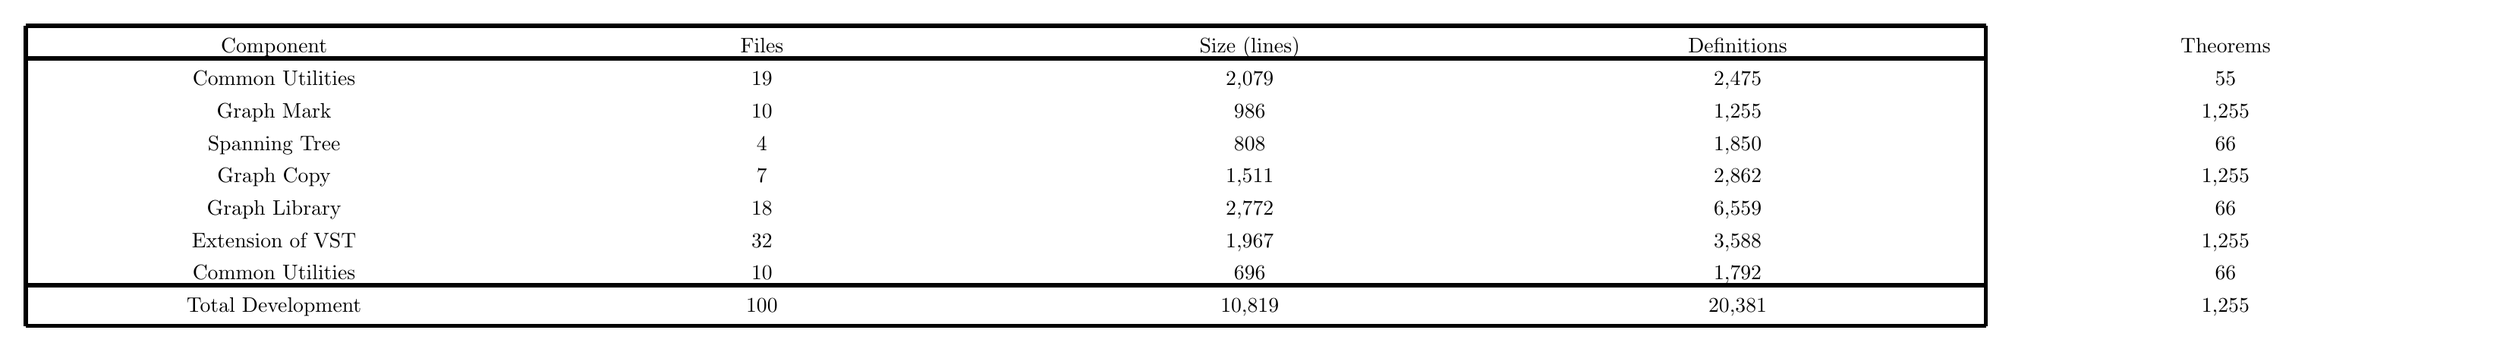
\begin{tikzpicture}[line width = 2pt]
  \matrix(stat)[
    matrix of nodes,
    ampersand replacement=\&,
    nodes={rectangle, align=center,text width=8cm},
    row sep=-\pgflinewidth,
    column sep=-\pgflinewidth,
    text depth=0.5ex,
    text height=2ex
  ]{
    |[fill=backgroundcolor]| Component \& |[fill=backgroundcolor]| Files \& |[fill=backgroundcolor]| Size (lines) \& |[fill=backgroundcolor]| Definitions \& |[fill=backgroundcolor]| Theorems \\
    Common Utilities  \& 19 \& 2,079 \& 2,475 \& 55 \\ 
    |[fill=backgroundcolor]| Graph Mark \& |[fill=backgroundcolor]| 10 \& |[fill=backgroundcolor]| 986 \& |[fill=backgroundcolor]| 1,255 \& |[fill=backgroundcolor]| 1,255 \\
    Spanning Tree  \& 4 \& 808 \& 1,850 \& 66 \\
    |[fill=backgroundcolor]| Graph Copy \& |[fill=backgroundcolor]| 7 \& |[fill=backgroundcolor]| 1,511 \& |[fill=backgroundcolor]| 2,862 \& |[fill=backgroundcolor]| 1,255\\
    Graph Library \& 18 \& 2,772 \& 6,559 \& 66\\
    |[fill=backgroundcolor]| Extension of VST  \& |[fill=backgroundcolor]| 32 \& |[fill=backgroundcolor]| 1,967 \& |[fill=backgroundcolor]| 3,588 \& |[fill=backgroundcolor]| 1,255\\
    Common Utilities \& 10 \& 696 \& 1,792 \& 66\\
    |[fill=backgroundcolor]| Total Development \& |[fill=backgroundcolor]| 100 \& |[fill=backgroundcolor]| 10,819 \& |[fill=backgroundcolor]| 20,381 \& |[fill=backgroundcolor]| 1,255\\
  };
  \draw(stat-1-1.north west)--(stat-1-4.north east);
  \draw(stat-2-1.north west)--(stat-2-4.north east);
  \draw(stat-9-1.north west)--(stat-9-4.north east);
  \draw(stat-9-1.south west)--(stat-9-4.south east);
  \draw(stat-1-1.north west)--(stat-9-1.south west);
  \draw(stat-1-4.north east)--(stat-9-4.south east);
\end{tikzpicture}
}}

  % \block{}{\centering\input{poster_pregraph.tex}}
  \block{}{
The structure of our Mathematical Graph Library.
The soundness condition is entirely customizable.
Lemmas and properties can be composed, and are automatically inherited.

\vspace{0.5em}
\hspace{-2.75ex}\centering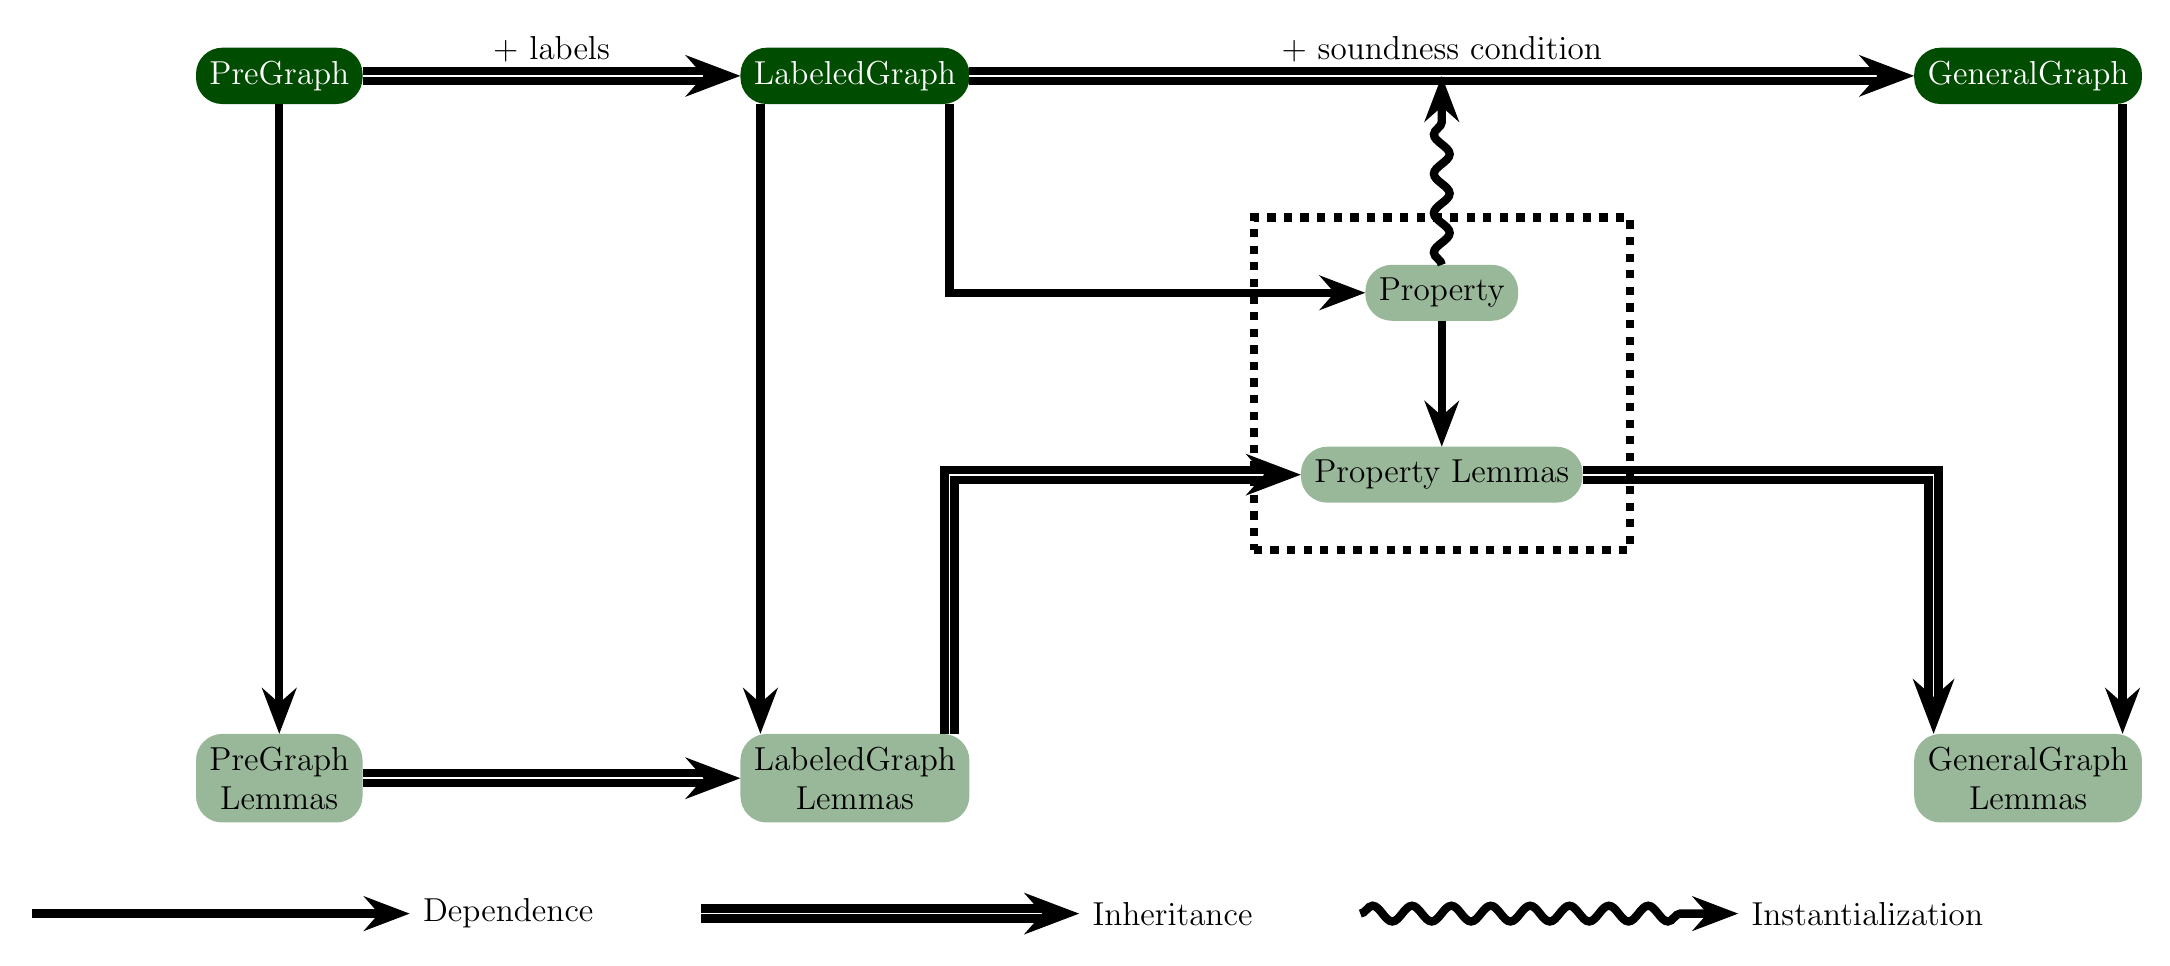
\begin{tikzpicture}
  [every shadow/.style={opacity=0.0, shadow xshift=8pt, shadow yshift=-8pt},
    ->/.style={line width=3pt, arrows={-Stealth}},
    -->/.style={line width=3pt, arrows={-Stealth}, decorate, decoration={snake, amplitude=1mm,segment length=5mm,post length=5mm}},
    realG/.style={shape=rectangle, rounded corners=8pt, text=white, draw=maincolor, fill=maincolor, drop shadow},
    propG/.style={shape=rectangle, rounded corners=8pt, text=black, draw=accentcolor, fill=accentcolor, drop shadow},
    x=6cm, y=4cm, line width=3pt, font=\large]
\node[realG] (PG) at (0, 0) { PreGraph};
\node[realG] (LG) [right=0.8 of PG] { LabeledGraph};
\node[realG] (GG) [right=2 of LG] { GeneralGraph};
\draw [double, ->] (PG) -- (LG) node [pos=0.5, above] { $+$ labels} ;
\draw [double, ->] (LG) -- (GG) node (SC) [pos=0.5, above, align=center]
{ $+$ soundness condition};
\node[propG] (Prop) [below=0.6 of SC] { Property};
\node[propG] (PropL) [below=0.4 of Prop] { Property Lemmas};
\node[propG] (PGL) [below=2 of PG, align=center] { PreGraph \\ Lemmas};
\node[propG] (LGL) [below=2 of LG, align=center] { LabeledGraph \\ Lemmas};
\node[propG] (GGL) [below=2 of GG, align=center] { GeneralGraph \\ Lemmas};
\draw [double, ->] (PGL) to (LGL);
%% \draw [double, ->] (LGL) to (GGL);
\draw [->] (PG) to (PGL);
\draw [->] (Prop) to (PropL);
\draw [-->] (Prop) to (SC);
\coordinate [left=0.2 of LG.south] (LGs1);
\coordinate [left=0.2 of LGL.north] (LGLn1);
\draw [->] (LGs1) to (LGLn1);
\coordinate [right=0.2 of LG.south] (LGs2);
\coordinate [right=0.2 of LGL.north] (LGLn2);
\draw [->] (LGs2) |- (Prop);
\draw [double, ->] (LGLn2) |- (PropL);
\coordinate [right=0.2 of GG.south] (GGs);
\coordinate [left=0.2 of GGL.north] (GGLn1);
\coordinate [right=0.2 of GGL.north] (GGLn2);
\draw [double, ->] (PropL) -| (GGLn1);
\draw [->] (GGs) to (GGLn2);
\node [draw, rectangle, dashed, inner sep=0.6cm, fit=(Prop) (PropL)] {};
\node (legend1) [below right=0.2 and 0.1 of PGL] { Dependence};
\coordinate[left=0.8 of legend1]  (l1);
\draw [->] (l1) to (legend1);
\node (legend2) [right=1 of legend1] { Inheritance};
\coordinate[left=0.8 of legend2]  (l2);
\draw [double, ->] (l2) to (legend2);
\node (legend3) [right=1 of legend2] { Instantialization};
\coordinate[left=0.8 of legend3]  (l3);
\draw [-->] (l3) to (legend3);
\end{tikzpicture}
% \captionof{figure}{Structure of the Mathematical Graph Library}
\vspace{-1.5em}}

\block{Instantiating \p{DijkGraph}}
{
\begin{flushleft}
% \begin{minipage}[c]{0.46\textwidth}
% \vspace*{-1ex}
\begin{equation*}
\begin{split}
\textbf{PreGraph: } &\texttt{VType := Z}, \texttt{ EType := Z * Z}, \texttt{ src := fst}, \texttt{ dst := snd},\\ 
                    &\forall \m{v}.~\texttt{vvalid}(\gamma, \m{v}) <=> 0 \le \m{v} < {\sz}, \\
                    &\forall \m{s,d}.~\texttt{evalid}(\gamma, \m{(s,d)}) <=> \texttt{vvalid}(\gamma, \m{s}) /| \texttt{vvalid}(\gamma, \m{d}) \\
\textbf{LabeledGraph: } &\texttt{ELType := Z}, \texttt{ VLType := list ELType}, \texttt{ GLType := unit} \\
\textbf{GeneralGraph: } &FiniteGraph(\gamma) /| \null \\
&\forall \m{i,j}.~\texttt{vvalid}(\gamma, \m{i}) /| \texttt{vvalid}(\gamma, \m{j}) => \\
&\qquad \m{i} = \m{j} => \texttt{elabel}(\gamma,(\m{i},{j})) = 0 /| \null \\
&\qquad \m{i} \neq \m{j} => 0 \le \texttt{elabel}(\gamma,(\m{i},{j})) \le \texttt{MAX/SIZE}
\end{split}
\end{equation*}
\end{flushleft}
\vspace{-1.5em}
}%end block

\block{Upper Bound on Path Cost}
{
The longest optimal path has \texttt{SIZE-1} links, so say we set \texttt{elabel}'s upper bound to $\lfloor\texttt{MAX/(SIZE-1)}\rfloor$. Consider the following example, where \texttt{MAX} = 7 and \texttt{SIZE} = 3, and so $0 \le \texttt{elabel}(\gamma, \m{e}) \le 3$. The check on line $20$ overflows when scanning C's neighbors: ($\lfloor\texttt{MAX/(SIZE-1)}\rfloor$ \texttt{ * (SIZE-1)}) + $\lfloor\texttt{MAX/(SIZE-1)}\rfloor$ \texttt{ > MAX}.
\vspace{0.5em}


{\centering
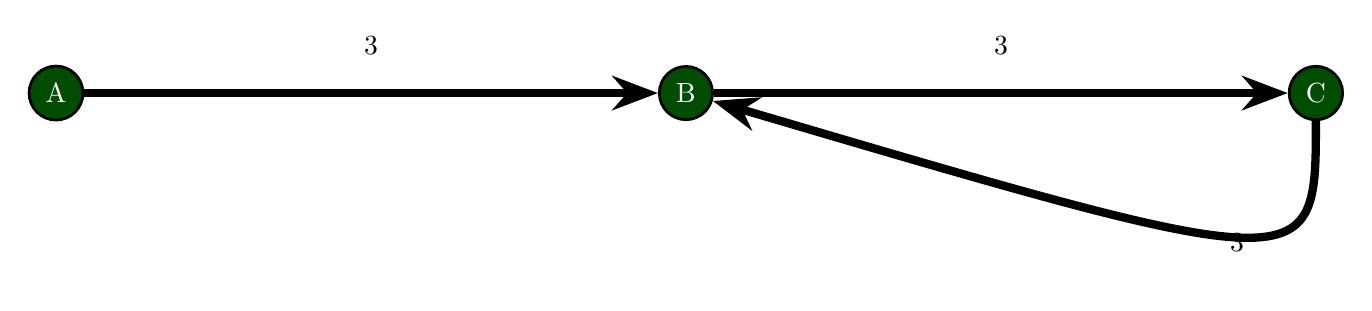
\begin{tikzpicture}[on grid,
  vert/.style={circle, line width=1pt, draw, fill=maincolor}]
  \node[vert] (A) at (0,0) {\color{white}A};
  \node[vert] (B) [right = 8 of A] {\color{white}B};
  \node[vert] (C) [right = 8 of B] {\color{white}C};
  \draw [->,line width=3pt,arrows={-Stealth}] (A) -- (B);
  \draw [->,line width=3pt,arrows={-Stealth}] (B) -- (C);
  \draw [->,line width=3pt,arrows={-Stealth}] (C.south) .. controls ++(0, -2) .. (B);
  \node at (4,0.6) {3};
  \node at (12,0.6) {3};
  \node at (15,-1.9) {3};
\end{tikzpicture}

}

Solution: Conservatively set the upper bound for an individual edge to
$\lfloor\texttt{MAX/SIZE}\rfloor$. 

New worst case: line $20$ calculates 
($\lfloor\texttt{MAX/SIZE}\rfloor$ \texttt{ * (SIZE-1)})\texttt{ + } $\lfloor\texttt{MAX/SIZE}\rfloor$ \texttt{ = MAX}.

The true maximum path cost is 
$\lfloor\texttt{MAX/SIZE}\rfloor$ \texttt{ * (SIZE-1) = MAX - } $\lfloor\texttt{MAX/SIZE}\rfloor$. 
}%end block

  \column{0.5}
  \block{Code and Specification}{\colorlet{stash}{red}
\colorlet{red}{maincolor}

\begin{lstlisting}
  void dijkstra (int graph[SIZE][SIZE], int src, 
                           int *dist, int *prev) {
$//$ $\braces{\p{DijkGraph}(\gamma)}$
    int pq[SIZE];
    int i, j, u, cost;
    for (i = 0; i < SIZE; i++) {
      dist[i] = INF; 
      prev[i] = INF; 
      pq[i] = INF;
    }
    dist[src] = 0; 
    pq[src] = 0; 
    prev[src] = src;
$//$ $\braces{\p{DijkGraph}(\gamma) /| \null \\
\m{dijk\_correct}(\gamma,\m{src},\m{prev},\m{dist},\m{priq})}$
    while (!pq_emp(pq)) {
      u = popMin(pq);
      for (i = 0; i < SIZE; i++) {
        cost = graph[u][i]; 
        if (cost < INF) {
          if (dist[i] > dist[u] + cost) {
            dist[i] = dist[u] + cost;
            prev[i] = u; 
            pq[i] = dist[i];
          }
        }  
      }
    }
$//$ $\braces{\p{DijkGraph}(\gamma) /| \null \\ 
\forall \m{dst} \in \m{priq}.~\m{priq}[\m{dst}] = \texttt{INF} /| \null \\ 
\m{dijk\_correct}(\gamma,\m{src},\m{prev},\m{dist},\m{priq})}$
    return;
  }
\end{lstlisting}
\vspace{0.5em}
\begin{equation*}
\begin{split}
\p{list\_rep}(\gamma, \m{i}) &\defeq \texttt{data\_at  array  graph2mat}(\gamma)[\m{i}] \texttt{  list\_addr}(\gamma, \m{i}) \\
\vspace{1em}
\p{graph\_rep}(\gamma) &\defeq \underset{\texttt{vvalid}(\gamma,\m{v})}{\bigstar} \m{v}  \mapsto\p{list\_rep}(\gamma, \m{v})
\end{split}
\end{equation*}

\begin{equation*}
\begin{split}
\m{dijk\_correct}(\gamma, \m{src}, \m{prev}, \m{dist},& \m{priq}) \; \defeq \; \\
\forall \m{dst}.~\m{dst} \in \m{popped}(\m{priq}) \; => \; & \exists \m{path}.~\m{path\_correct}(\gamma, \m{prev}, \m{dist}, \m{path}) /| \null \\
& \m{path\_glob\_optimal}(\gamma, \m{dist}, \m{path}) /| \null \\
& \m{path\_entirely\_in\_popped}(\gamma, \m{prev}, \m{path}) /| \null \\
\m{priq}[\m{dst}] < \ifty \; => \; & \texttt{let }\m{m} \texttt{ := } \m{prev}[\m{dst}] \texttt{ in } \m{m} \in \m{popped}(\m{priq}) /| \null \\
&\forall \m{m'} \in \m{popped}(\m{priq}).~\m{cost}(\m{path2m} +:: (m, dst)) \le \null \\
&\hspace{10em} \m{cost}(\m{path2m'} +:: (m', dst)) /| \null \\
\m{priq}[\m{dst}] = \ifty \; => \; & \forall \m{m} \in \m{popped}(\m{priq}).~\m{cost}(\m{path2m} +:: (m, dst)) = \ifty
\end{split}
\end{equation*}

\colorlet{red}{stash}

  \vspace{-1.5em}
}

\newcommand{\s}{11}
\colorlet{midaccentcolor}{titlebgcolor!80!white}

\block{Key Transformation: Growing the Subgraph} {

{\centering
\begin{tikzpicture}[on grid,
  popped/.style={rounded corners=50pt, line width=1pt, draw, fill=maincolor},
  fringe/.style={rounded corners=50pt, line width=1pt, draw, fill=accentcolor},
  popping/.style={rounded corners=50pt, line width=1pt, draw, dashed, fill=midaccentcolor},
  unseen/.style={rounded corners=50pt, line width=1pt, draw}]
  \draw[unseen] (0,0) -- (\s,0) -- (\s,\s) -- (0,\s) -- cycle;
  \draw[fringe] (1.5,1.5) -- (9.5,1.5) -- (9.5,9.5) -- (1.5,9.5) -- cycle;
  \draw[popped] (3,3) -- (8,3) -- (6,6) -- (3,8) -- cycle;
  \node at (1.4,1) {dst$_3$};   
  \node at (2.9,2.5) {dst$_2$};   
  \node at (4.4,4) {\color{white}dst$_1$}; 
  \node at (6.6,7) {u};
\tikzset{shift={(13.5,0)}}

  \draw[unseen] (0,0) -- (\s,0) -- (\s,\s) -- (0,\s) -- cycle;
  \draw[fringe] (1.5,1.5) -- (9.5,1.5) -- (9.5,9.5) -- (1.5,9.5) -- cycle;
  \draw[popping] (3,3) -- (8,3) -- (8,8) -- (3,8) -- cycle;
  \draw[popped] (3,3) -- (8,3) -- (6,6) -- (3,8) -- cycle;
  \node at (1.4,1) {dst$_3$};   
  \node at (2.9,2.5) {dst$_2$};   
  \node at (4.4,4) {\color{white}dst$_1$}; 
  \node at (6.6,7) {u};     

\tikzset{shift={(13.5,0)}}

  \draw[unseen] (0,0) -- (\s,0) -- (\s,\s) -- (0,\s) -- cycle;
  \draw[fringe] (1.5,1.5) -- (9.5,1.5) -- (9.5,9.5) -- (1.5,9.5) -- cycle;
  \draw[popped] (3,3) -- (8,3) -- (8,8) -- (3,8) -- cycle;
  \node at (1.4,1) {dst$_3$};   
  \node at (2.9,2.5) {dst$_2$};   
  \node at (4.4,4) {\color{white}dst$_1$}; 
  \node at (6.6,7) {\color{white}u};       
\end{tikzpicture}

}% end centering

\vspace{0.5em}

To begin, vertices dst$_1$, dst$_2$, and dst$_3$ obey the first, second, and third 
clauses of the invariant \m{dijk\_correct} respectively. Vertex u obeys the second clause with minimal cost. 

\vspace{0.5em}

The invariant is broken when relaxing u's neighbors, and reestablished thereafter:~u now obeys the first clause. Eventually no vertices obey the second clause, and we are done.
\vspace{-1.5em}
}% end block

\block{References}{
    \printbibliography[heading=none]
}
\end{columns}
\end{document}
